% EMBC 2026 A0 portrait poster — native LaTeX source.
% Build with: make
% Physical canvas: 841 mm x 1189 mm (true A0 portrait).
\documentclass[final]{beamer}
\usepackage[size=a0,orientation=portrait,scale=1.0]{beamerposter}
\usepackage{fontspec}
\usepackage{microtype}
\usepackage{graphicx}
\usepackage{booktabs}
\usepackage{tabularx}
\usepackage{array}
\usepackage{amsmath,amssymb}
\usepackage{siunitx}
\usepackage[most]{tcolorbox}
\usepackage{tikz}
\usepackage{ragged2e}
\usepackage{qrcode}
\usepackage{hyperref}

\defaultfontfeatures{Ligatures=TeX}
\setsansfont{TeX Gyre Heros}
\setmainfont{TeX Gyre Heros}
\usefonttheme{professionalfonts}

\definecolor{IEEEBlue}{HTML}{00629B}
\definecolor{DeepNavy}{HTML}{17324D}
\definecolor{SignalTeal}{HTML}{00A6A6}
\definecolor{WarmGold}{HTML}{F2B134}
\definecolor{MistBlue}{HTML}{E9F4FA}
\definecolor{PaleGold}{HTML}{FFF4D6}
\definecolor{Ink}{HTML}{172B3A}
\definecolor{Muted}{HTML}{536273}
\definecolor{Rule}{HTML}{D8E1E8}

\hypersetup{colorlinks=true,urlcolor=IEEEBlue}
\setbeamertemplate{navigation symbols}{}
\setbeamercolor{background canvas}{bg=white}
\setbeamercolor{normal text}{fg=Ink,bg=white}
\setbeamersize{text margin left=13mm,text margin right=13mm}
\setlength{\columnsep}{12mm}
\setlength{\columnseprule}{0pt}
\setlength{\parindent}{0pt}
\setlength{\parskip}{3mm}
\renewcommand{\arraystretch}{1.12}

\newcommand{\BodyFont}{\fontsize{25}{30}\selectfont}
\newcommand{\SmallFont}{\fontsize{21}{25}\selectfont}
\newcommand{\TinyFont}{\fontsize{18}{22}\selectfont}
\newcommand{\CaptionFont}{\fontsize{18}{22}\selectfont}
\newcommand{\HeadingFont}{\fontsize{40}{44}\selectfont\bfseries}
\newcommand{\SubheadingFont}{\fontsize{29}{34}\selectfont\bfseries}
\newcommand{\Metric}[2]{%
  \begin{minipage}[c]{0.235\linewidth}\centering
    {\fontsize{47}{50}\selectfont\bfseries\color{DeepNavy}#1}\\[-1mm]
    {\fontsize{19}{23}\selectfont\color{Muted}#2}
  \end{minipage}}

\newtcolorbox{PosterBox}[2][]{%
  enhanced,
  colback=white,
  colframe=Rule,
  boxrule=1.1pt,
  arc=4mm,
  left=6mm,right=6mm,top=5mm,bottom=5mm,
  before skip=5mm,after skip=5mm,
  title={#2},
  fonttitle=\HeadingFont,
  coltitle=white,
  colbacktitle=IEEEBlue,
  boxed title style={arc=3mm,boxrule=0pt},
  attach boxed title to top left={xshift=0mm,yshift=-1mm},
  #1
}
\newtcolorbox{GoldBox}[1][]{%
  enhanced,colback=PaleGold,colframe=WarmGold,boxrule=1.4pt,arc=4mm,
  left=6mm,right=6mm,top=5mm,bottom=5mm,
  before skip=5mm,after skip=5mm,#1
}
\newtcolorbox{TealBox}[1][]{%
  enhanced,colback=MistBlue,colframe=SignalTeal,boxrule=1.4pt,arc=4mm,
  left=6mm,right=6mm,top=5mm,bottom=5mm,
  before skip=5mm,after skip=5mm,#1
}

\newcolumntype{Y}{>{\RaggedRight\arraybackslash}X}
\newcolumntype{C}[1]{>{\centering\arraybackslash}p{#1}}
\newcommand{\yes}{\textcolor{SignalTeal}{\bfseries 1}}
\newcommand{\no}{\textcolor{Muted}{0}}

% Replace these two macros with the authors' confirmed wording before printing.
\newcommand{\FundingStatement}{\textbf{Author confirmation required:} insert all financial support and collaborations before printing. No funding statement was present in the supplied materials.}
\newcommand{\ConflictStatement}{\textbf{Conflict-of-interest statement:} author confirmation required before printing.}
\newcommand{\PosterNumber}{Poster D-12}

\begin{document}
\begin{frame}[t]

% Official template motifs, used faintly so they do not compete with the data.
\begin{tikzpicture}[remember picture,overlay]
  \node[anchor=north west,opacity=0.22] at ([xshift=-4mm,yshift=-145mm]current page.north west)
    {
\includegraphics[height=800mm]{assets/template/image1.png}};
  \node[anchor=south east,opacity=0.20] at ([xshift=2mm,yshift=15mm]current page.south east)
    {
\includegraphics[height=650mm]{assets/template/image3.png}};
\end{tikzpicture}

% Header
\begin{columns}[T,totalwidth=\textwidth]
  \begin{column}{0.145\textwidth}
    \centering
    
\includegraphics[width=0.92\linewidth]{assets/logos/embc2026.png}
  \end{column}
  \begin{column}{0.705\textwidth}
    \centering
    {\fontsize{76}{82}\selectfont\bfseries\color{DeepNavy}
      Benchmarking Loss Functions for 12-Lead ECG Reconstruction from Limited Leads\par}
    \vspace{3mm}
    {\fontsize{46}{52}\selectfont\bfseries\color{IEEEBlue}
      A Multi-Objective Framework for Morphological Fidelity\par}
    \vspace{6mm}
    {\fontsize{34}{40}\selectfont\bfseries
      Mithun Manivannan \enspace$\cdot$\enspace Alex Mariakakis
      \enspace$\cdot$\enspace Christopher Cheung\par}
    \vspace{2mm}
    {\fontsize{26}{31}\selectfont\color{Muted}
      Sunnybrook Health Sciences Centre \enspace$\cdot$\enspace
      University of Toronto \enspace$\cdot$\enspace Toronto, Canada\par}
  \end{column}
  \begin{column}{0.15\textwidth}
    \centering
    \vspace{15mm}
    
\includegraphics[width=0.96\linewidth]{assets/logos/ieee_embs.png}
  \end{column}
\end{columns}

\vspace{7mm}
\begin{TealBox}
  \centering
  {\fontsize{36}{42}\selectfont\bfseries\color{DeepNavy}
    Point-wise accuracy is necessary but not sufficient:
    \textcolor{IEEEBlue}{MSE anchors amplitude}, correlation improves morphology
    \emph{when calibrated}, and the best combination is architecture-dependent.\par}
  \vspace{5mm}
  \Metric{48}{primary factorial models}\hfill
  \Metric{2,198}{held-out PTB-XL ECGs}\hfill
  \Metric{17}{paired stress conditions}\hfill
  \Metric{3}{external/device cohorts}
\end{TealBox}

\vspace{2mm}
\begin{columns}[T,totalwidth=\textwidth]

% ========================= COLUMN 1 =========================
\begin{column}{0.31\textwidth}
\begin{PosterBox}{Introduction \& Objective}
\BodyFont
Reconstructing a clinical 12-lead ECG from leads \textbf{I, II, and V2} is
underdetermined. A model can achieve high global correlation while distorting
amplitude, QRS slopes, ST morphology, or downstream classifier outputs.

\textbf{Question.} Across U-Net, MultiScale-VAE, and ECG-AIM, what does each
loss component contribute to waveform fidelity, morphology, robustness, and
diagnostic preservation?

\begin{GoldBox}[before skip=3mm,after skip=0mm]
\SubheadingFont\color{DeepNavy}Core hypothesis\par
\BodyFont
The losses are \textbf{complementary constraints}, not interchangeable
surrogates. Their effects should therefore be estimated factorially and
separately for each architecture.
\end{GoldBox}
\end{PosterBox}

\begin{PosterBox}{Loss Anatomy: Complete \texorpdfstring{$2^4$}{2-to-the-4} Objective}
\BodyFont
For target ECG \(y\), reconstruction \(\hat y\), \(L\) leads and \(T\) time
samples, each binary mask \(E/C/M/D\) activates one term:
\[
\boxed{\mathcal L =
E\,\mathcal L_{\mathrm{MSE}}
0.5C\,\mathcal L_{\mathrm{corr}}
0.1M\,\mathcal L_{\mathrm{MMD}}
0.05D\,\mathcal L_{\Delta}}
\]
\vspace{-5mm}
\begin{align*}
\mathcal L_{\mathrm{MSE}}
  &= \frac{1}{LT}\lVert y-\hat y\rVert_2^2
  &&\text{\color{IEEEBlue}{amplitude calibration}}\\
\mathcal L_{\mathrm{corr}}
  &= 1-\frac{1}{L}\sum_{\ell=1}^{L}\rho(y_\ell,\hat y_\ell)
  &&\text{\color{IEEEBlue}{shape / phase alignment}}\\
\mathcal L_{\Delta}
  &= \operatorname{MSE}(\Delta y,\Delta\hat y)
  &&\text{\color{IEEEBlue}{slope preservation}}\\
\mathcal L_{\mathrm{MMD}}
  &= \mathbb E k(\hat y,\hat y')+\mathbb E k(y,y')\\[-1mm]
  &\quad -2\mathbb E k(\hat y,y')
  &&\text{\color{IEEEBlue}{distribution matching}}
\end{align*}
\SmallFont
MMD uses four scale-adaptive RBF kernels with bandwidth multipliers
\(\{0.5,1,2,4\}\) around the detached median batch distance. Distances are
mean-squared per feature, preventing kernel underflow at ECG dimensionality.

\vspace{2mm}
\centering
\begin{tabular}{C{31mm}C{31mm}C{31mm}C{31mm}l}
\toprule
\textbf{E} & \textbf{C} & \textbf{M} & \textbf{D} & \textbf{Mask example}\\
\midrule
\yes & \no & \no & \no & MSE-only \(1000\)\\
\yes & \yes & \yes & \yes & full \(1111\)\\
\no & \yes & \yes & \yes & no-MSE \(0111\)\\
\bottomrule
\end{tabular}
\end{PosterBox}

\begin{PosterBox}{Experimental Design}
\SmallFont
\begin{tabularx}{\linewidth}{>{\bfseries\color{DeepNavy}}p{44mm}Y}
\toprule
Factorial grid & 3 architectures \(\times\) 16 E/C/M/D masks \(=48\) seed-42 runs\\
Confirmation & 18 runs: base, full, and validation-selected configurations at seeds 1337 and 2026\\
Input / target & I, II, V2 observed; nine missing leads evaluated primarily\\
Checkpoint rule & Lowest missing-lead validation MSE; Pearson tie-breaker\\
Clean test & PTB-XL fold 10: 2,198 ECGs from 1,904 patients\\
Statistics & 2,000 paired patient-cluster BCa resamples; \(\alpha=0.0167\) for QRS, ST, diagnostic utility\\
Stress test & Gaussian + NSTDB BW/EM/MA at 24/12/6/0 dB, plus synthetic baseline drift\\
External/device & EchoNext \(n=5{,}442\); smartwatch \(n=719\); Sunnybrook Cath Lab \(n=20\)\\
Frozen readouts & ECGFounder 150-task, five PTB-XL superclasses, and signal-quality head\\
\bottomrule
\end{tabularx}
\vspace{2mm}
\CaptionFont\color{Muted}
Observed leads are preserved exactly by the unified adapter. Identical ECG IDs
and deterministic noise realizations are used for paired comparisons.
\end{PosterBox}

\begin{PosterBox}{Evaluation Contract}
\SmallFont
\begin{itemize}
  \setlength{\itemsep}{2mm}
  \item \textbf{Signal:} MSE, RMSE, MAE, \(R^2\), Pearson, SNR, derivative error.
  \item \textbf{Morphology:} standardized QRS \([-50,+100]\) ms; ST \([+120,+240]\) ms; J-point and R-peak timing.
  \item \textbf{Utility:} AUROC, AP, F1, ECE, Brier, subgroup gaps.
  \item \textbf{Transfer:} physical units and source sampling preserved; no per-record min--max transform.
\end{itemize}
\end{PosterBox}

\begin{PosterBox}{Model Families \& Reproducibility}
\SmallFont
\begin{tabularx}{\linewidth}{>{\bfseries}Y C{31mm} C{29mm} Y}
\toprule
Family & Batch & Epochs & Role in design\\
\midrule
U-Net & 256 & 10 & deterministic convolutional baseline\\
MultiScale-VAE & 32 & 10 & variational, multi-resolution decoder\\
ECG-AIM & 32 & 10 & learned-token latent reconstruction\\
\bottomrule
\end{tabularx}
\vspace{4mm}
\begin{tabularx}{\linewidth}{C{12mm}Y}
\textcolor{SignalTeal}{\Large\(\checkmark\)} & 48/48 primary checkpoints load through one adapter\\
\textcolor{SignalTeal}{\Large\(\checkmark\)} & finite \([B,12,5000]\) output and exact observed-lead passthrough\\
\textcolor{SignalTeal}{\Large\(\checkmark\)} & 2,198 clean records and 17 stress conditions per cell\\
\textcolor{SignalTeal}{\Large\(\checkmark\)} & strict JSON, per-record Parquet, source hashes, and 22/22 package checks\\
\end{tabularx}
\end{PosterBox}
\end{column}

% ========================= COLUMN 2 =========================
\begin{column}{0.35\textwidth}
\begin{PosterBox}{Results I: the 48-Cell Loss Landscape}
\centering
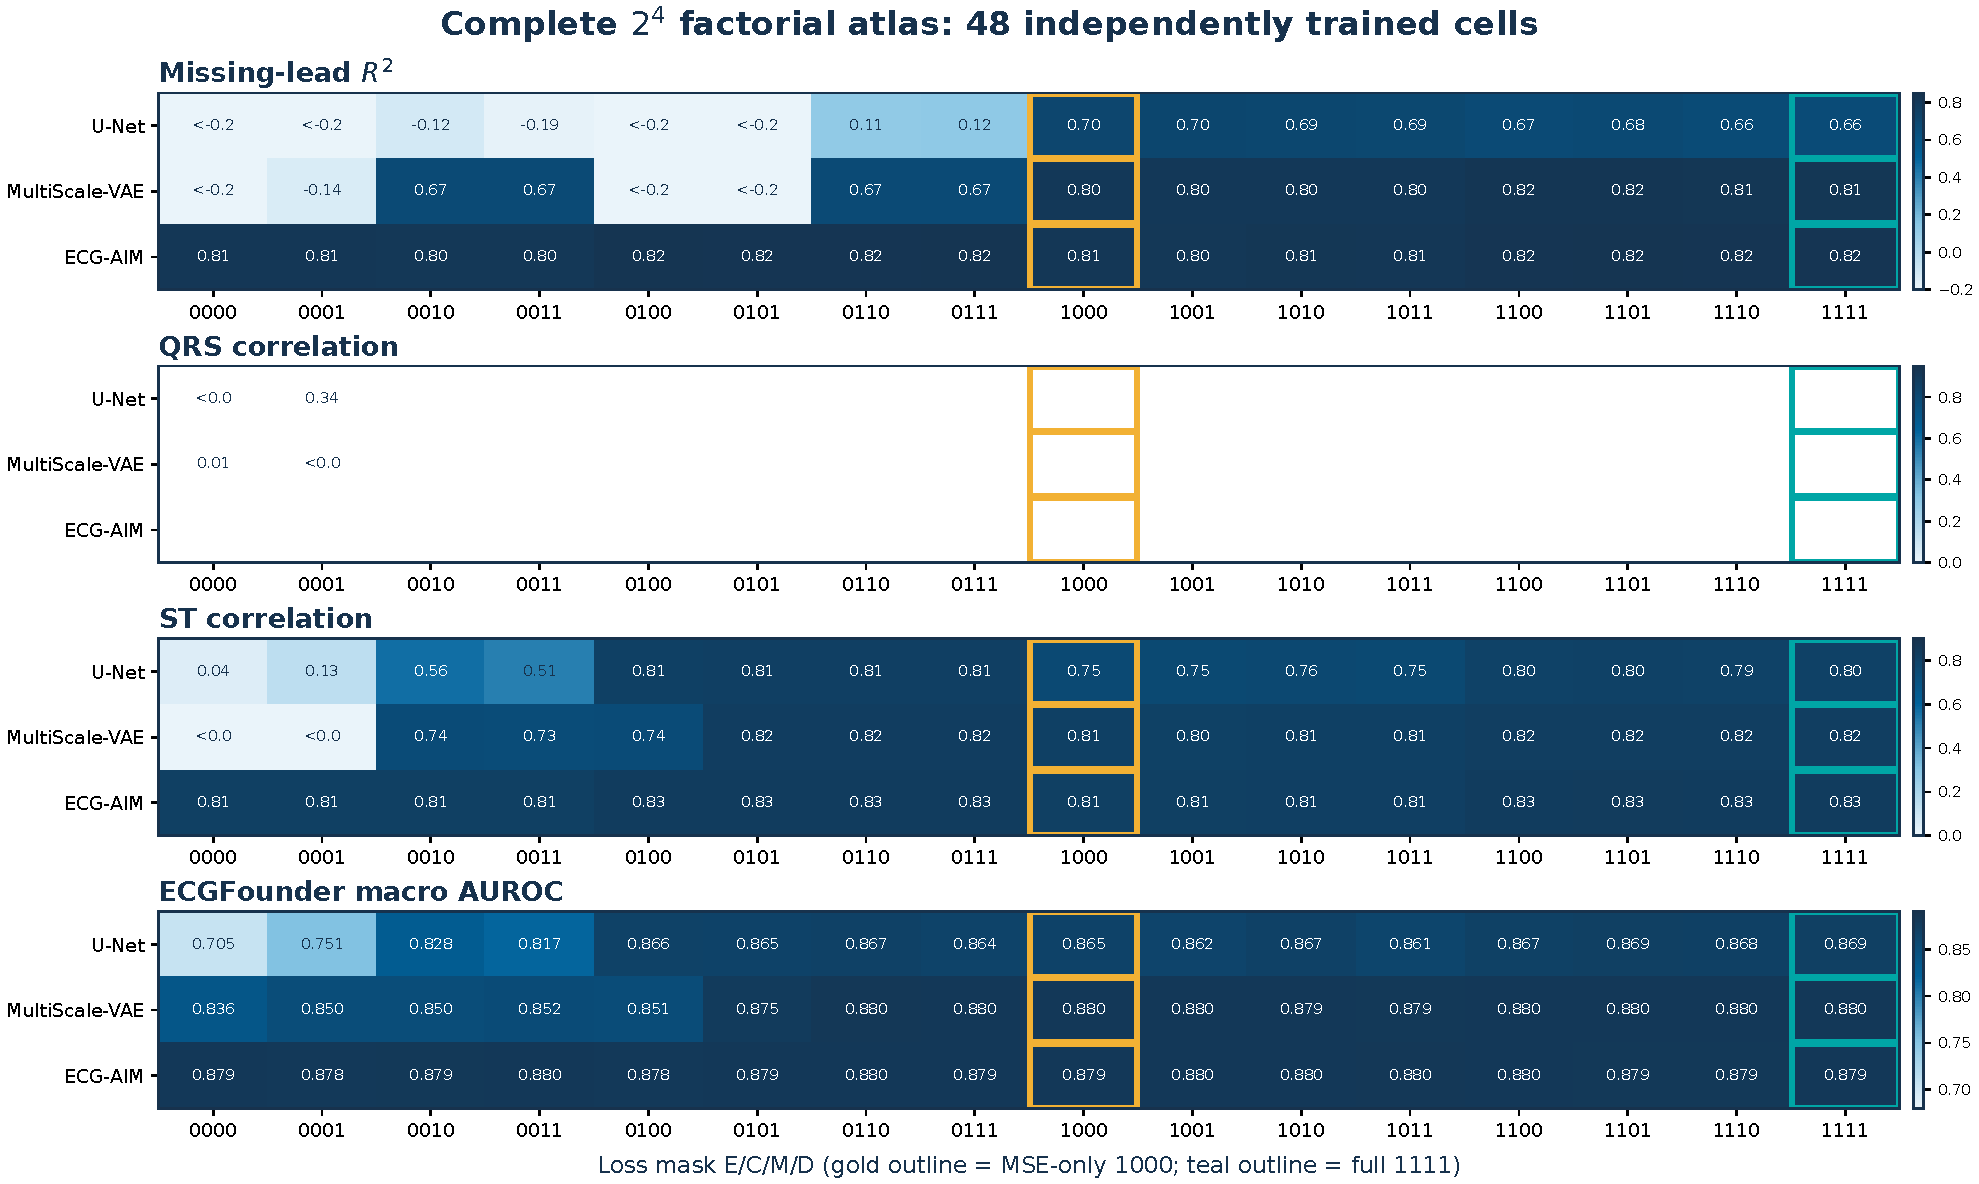
\includegraphics[width=\linewidth]{assets/figures/factorial_atlas.pdf}
\CaptionFont\color{Muted}
\textbf{Figure 1.} Complete E/C/M/D grid. The MSE-off half exposes severe
calibration failures in U-Net and MultiScale-VAE; ECG-AIM is substantially
less sensitive. Gold = prespecified MSE-only; teal = full composite.
\end{PosterBox}

\begin{PosterBox}{Results II: Clinical Endpoint Tests}
\centering
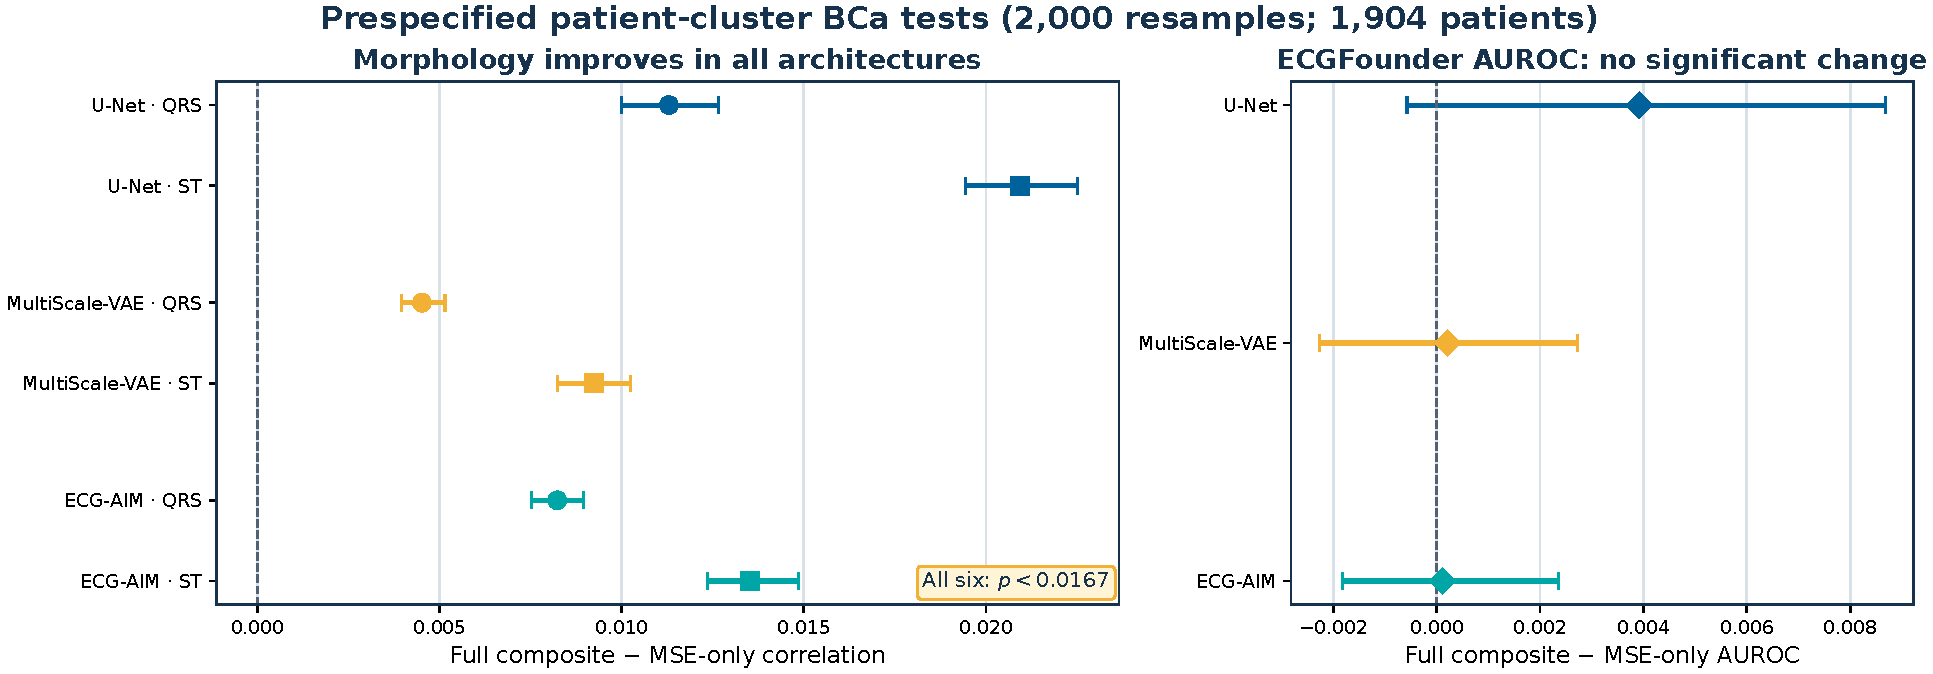
\includegraphics[width=\linewidth]{assets/figures/clinical_effects.pdf}
\CaptionFont\color{Muted}
\textbf{Figure 2.} Full composite versus MSE-only. All six QRS/ST contrasts
improve at the family-wise threshold. ECGFounder AUROC intervals cross zero in
all architectures: no significant change, \emph{not} proof of equivalence.

\begin{GoldBox}[before skip=4mm,after skip=0mm]
\BodyFont
\textbf{\color{DeepNavy}Critical failure mode.}
MultiScale-VAE mask \(0100\) (correlation only) attains Pearson
\(\rho=0.874\) but \(R^2=-14.984\). Correlation can recover shape while
allowing catastrophic scale error; \textbf{MSE is the calibration anchor}.
\end{GoldBox}
\end{PosterBox}

\begin{PosterBox}{Architecture-Specific Best Cells}
\SmallFont
\centering
\begin{tabular}{lcccc}
\toprule
\textbf{Family} & \textbf{Best \(R^2\) mask} & \textbf{\(R^2\)} &
\textbf{Full QRS} & \textbf{Full ST}\\
\midrule
U-Net & 1000 & 0.700 & 0.929 & 0.798\\
MultiScale-VAE & 1101 & 0.816 & 0.940 & 0.822\\
ECG-AIM & 0111 & \textbf{0.822} & \textbf{0.942} & \textbf{0.832}\\
\bottomrule
\end{tabular}
\par
\vspace{3mm}
\RaggedRight
\BodyFont
There is \textbf{no universal winning mask}. U-Net favors MSE-only for
\(R^2\); MultiScale-VAE favors MSE+correlation+derivative; ECG-AIM's best
\(R^2\) is achieved without MSE. Endpoint choice must be declared before
selecting a loss.
\end{PosterBox}

\begin{PosterBox}{Representative External Reconstructions}
\centering
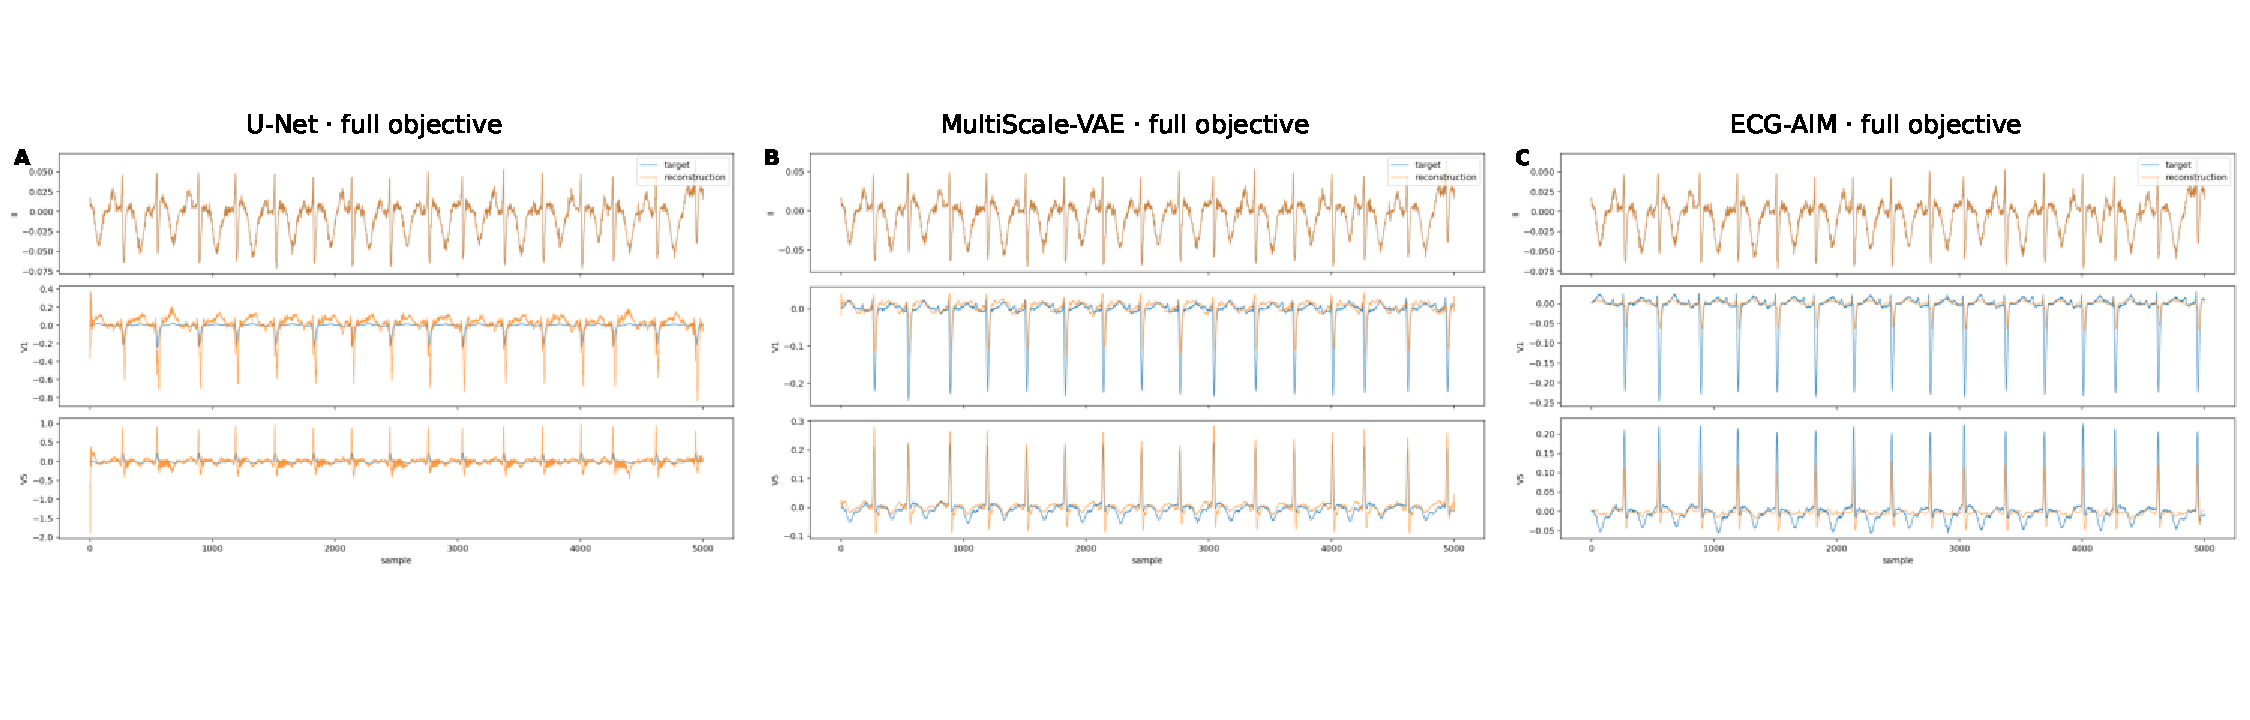
\includegraphics[width=\linewidth]{assets/figures/echonext_representative_reconstructions.pdf}
\CaptionFont\color{Muted}
\textbf{Figure 3.} EchoNext targets (blue) and full-loss reconstructions
(orange). Trace inspection reveals architecture-specific amplitude and
morphology errors that aggregate metrics alone can hide.
\end{PosterBox}

\begin{PosterBox}{Conditional Component Effects}
\centering
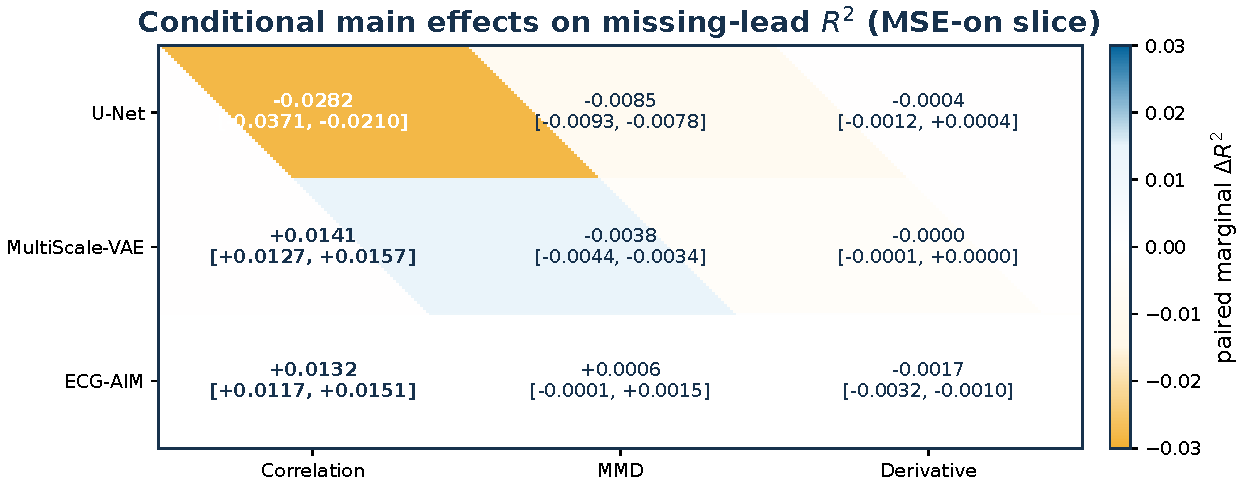
\includegraphics[width=0.94\linewidth]{assets/figures/conditional_r2_effects.pdf}
\CaptionFont\color{Muted}
\textbf{Figure 4.} Paired marginal effects within the prespecified MSE-on
\(2^3\) slice. Correlation lowers U-Net \(R^2\) but raises MultiScale-VAE and
ECG-AIM \(R^2\); this sign reversal is direct evidence against a universal
auxiliary-loss recipe. Values show estimate and 95\% BCa interval.
\end{PosterBox}

\end{column}

% ========================= COLUMN 3 =========================
\begin{column}{0.31\textwidth}
\begin{PosterBox}{Results III: Noise Robustness}
\centering
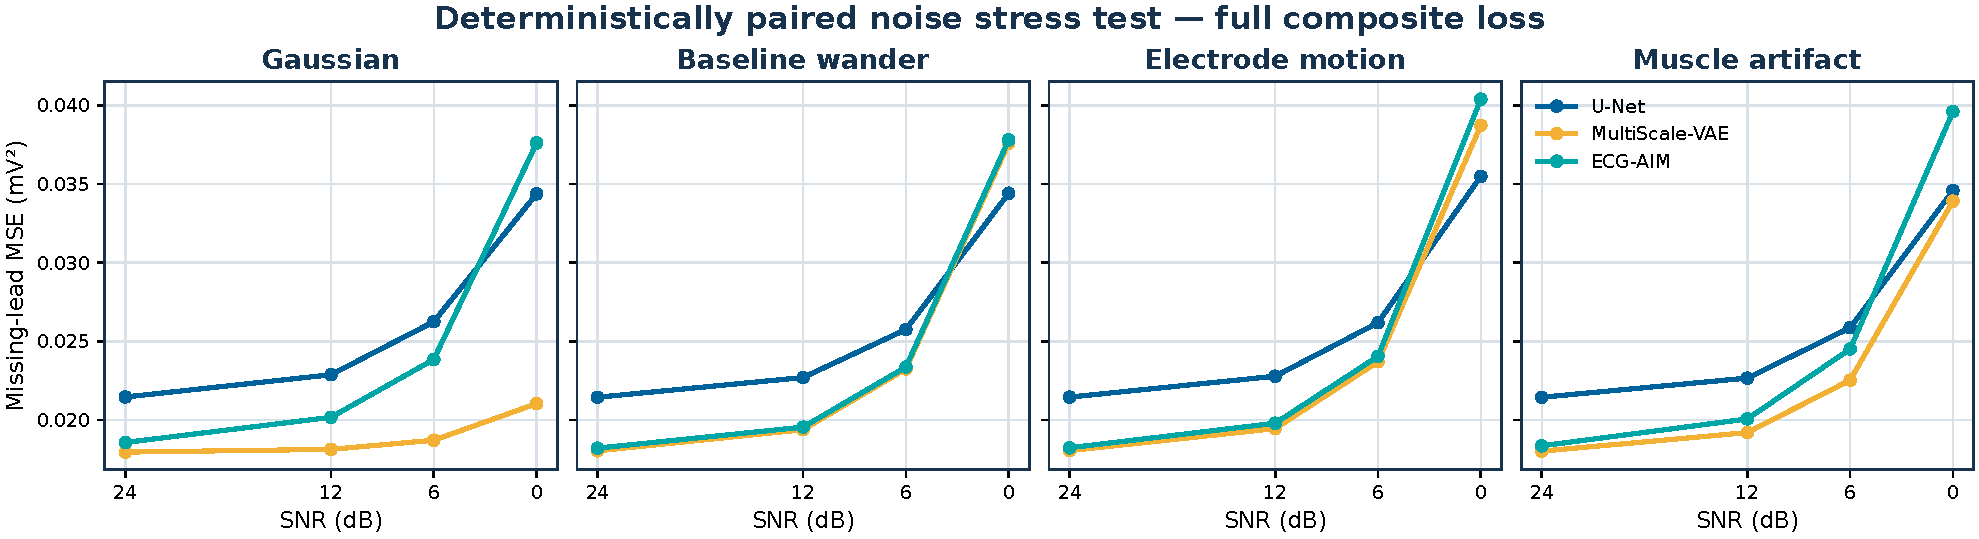
\includegraphics[width=\linewidth]{assets/figures/noise_stress.pdf}
\CaptionFont\color{Muted}
\textbf{Figure 5.} Identical paired noise realizations for each model.
MultiScale-VAE has the lowest full-loss missing-lead MSE across the plotted
stress curves, while all families degrade monotonically as SNR falls.
\end{PosterBox}

\begin{PosterBox}{Results IV: External Transfer}
\centering
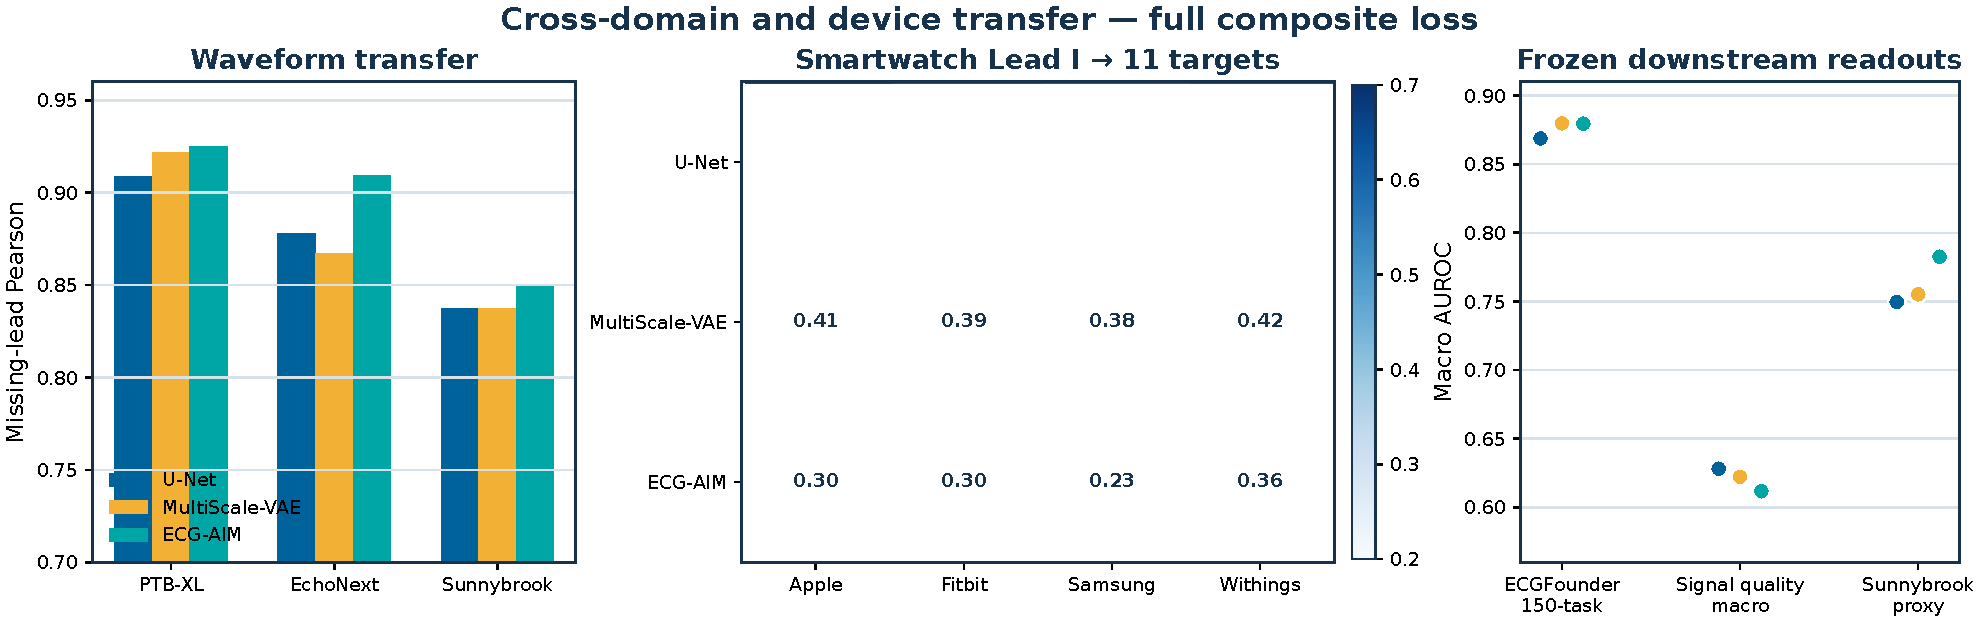
\includegraphics[width=\linewidth]{assets/figures/external_scorecard.pdf}
\CaptionFont\color{Muted}
\textbf{Figure 6.} Full-loss models across waveform, device, and frozen
downstream endpoints. EchoNext and Sunnybrook reveal smaller but still strong
waveform transfer; single-lead smartwatch transfer is strongly
architecture-dependent.

\begin{GoldBox}[before skip=4mm,after skip=0mm]
\SmallFont
\textbf{\color{DeepNavy}Scope matters.}
Smartwatch signals are calibrated simulator/device recordings, not a human
pathology cohort. Sunnybrook superclass AUROC uses non-adjudicated Philips
statement proxies; ECGFounder there is probability fidelity only.
\end{GoldBox}
\end{PosterBox}

\begin{PosterBox}{Diagnostic \& Signal-Quality}
\SmallFont
\begin{tabularx}{\linewidth}{>{\bfseries}Y C{31mm} C{31mm} C{31mm}}
\toprule
Full-loss endpoint & U-Net & MS-VAE & ECG-AIM\\
\midrule
ECGFounder macro AUROC & 0.869 & \textbf{0.880} & 0.879\\
PTB-XL quality macro AUROC & \textbf{0.628} & 0.622 & 0.612\\
Any-artifact AUROC & 0.683 & 0.683 & \textbf{0.697}\\
Quality probability fidelity & 0.806 & 0.893 & \textbf{0.934}\\
Sunnybrook Pearson & 0.838 & 0.839 & \textbf{0.849}\\
\bottomrule
\end{tabularx}
\vspace{3mm}
\BodyFont
Across all 48 cells, 27 meet the exploratory ECGFounder non-inferiority margin
of 0.02: ECG-AIM 16/16, MultiScale-VAE 11/16, U-Net 0/16. Signal-quality
electrode-problem AUROC remains exploratory because fold 10 has only three
positives.
\end{PosterBox}

\begin{PosterBox}{Discussion}
\BodyFont
\begin{enumerate}
  \setlength{\itemsep}{3mm}
  \item \textbf{MSE governs identifiability of scale.} Shape-only objectives
        can look convincing under Pearson correlation while being physically wrong.
  \item \textbf{Correlation supplies the strongest morphology signal} on the
        MSE-on slice, but its \(R^2\) effect changes sign by architecture.
  \item \textbf{Auxiliary terms interact.} Marginal effects cannot be
        transferred blindly between a convolutional U-Net, a variational
        multi-scale model, and ECG-AIM.
  \item \textbf{Utility is comparatively stable.} Morphology improves with
        the full objective without a significant ECGFounder AUROC shift, but
        this is not a clinical-safety claim.
\end{enumerate}
\end{PosterBox}

\begin{TealBox}
\HeadingFont\color{DeepNavy}Conclusion\par
\BodyFont
\textbf{Benchmark losses as experimental factors—not as a single leaderboard.}
For limited-lead ECG reconstruction, a calibrated point-wise anchor plus
explicit morphology constraints is the safest default, followed by
architecture- and endpoint-specific validation.
\end{TealBox}

\begin{PosterBox}{Limitations, Declaration \& Access}
\TinyFont
\textbf{Limitations.} Confirmation seeds cover only the MSE-on
base/full/selected slice. EchoNext diagnostic outputs retain tabular metadata.
Smartwatch inputs are simulator/device signals. Sunnybrook labels are
device-statement proxies. This benchmark evaluates reconstruction fidelity and
frozen readouts, not clinical deployment safety.

\textbf{Financial support / collaboration.} \FundingStatement

\textbf{Declaration of interest.} \ConflictStatement

\vspace{3mm}
\begin{columns}[c,totalwidth=\linewidth]
  \begin{column}{0.76\linewidth}
    \TinyFont
    \textbf{Data and provenance:} PTB-XL, NSTDB, EchoNext, the PhysioNet
    ECG-capable smartwatch database, and measured Sunnybrook Cath Lab ECGs.
    Exact machine-readable results, per-record tables, scripts, and hashes are
    included in the project repository.\\[2mm]
    \url{github.com/whiteblaze143/benchmarking_loss_functions_ecg_reconstruction}
  \end{column}
  \begin{column}{0.22\linewidth}
    \centering
    
\includegraphics[width=0.90\linewidth]{assets/qr/project_qr.png}
  \end{column}
\end{columns}
\end{PosterBox}
\end{column}
\end{columns}

\vfill
\begin{tcolorbox}[
  colback=DeepNavy,colframe=DeepNavy,boxrule=0pt,arc=0mm,
  left=8mm,right=8mm,top=4mm,bottom=4mm]
  \color{white}\fontsize{21}{25}\selectfont
  \textbf{IEEE EMBC 2026 \enspace|\enspace Toronto, Canada \enspace|\enspace
  26--30 July 2026}
  \hfill \PosterNumber
\end{tcolorbox}

\end{frame}
\end{document}
